\section{Method}
Time has not yet allowed for the creation of a neat and detailed test plan. However, before the voltage regulator boards are soldered onto the main board, they need to be thoroughly tested to verify their functionality. The plan is to create a test table for this purpose, similar to the specification of ICs in datasheets.

\subsection{Hardware}
\subsubsection{Voltage regulators}
For the voltage regulator modules, the following parameters need to be measured to demonstrate proper operation:
-Thorough visual inspection, especially focusing on the soldering process. This includes checking for short circuits, open connections, solder balls, and other defects.
-The converter should be powered from a lab power supply with low current limit settings. In case of a short circuit or other module defect, the dissipated power will be limited, allowing for the identification and resolution of the issue.
-The output voltage of the converter should be observed using an oscilloscope. Attention should be paid to the absolute accuracy and the amplitude of the ripple voltage.
-The temperature of the PCBA should be monitored to ensure that the module does not get too hot, which could potentially shorten its lifespan.

\subsubsection{Main board}
The functionality of the main board should be verified in the following manner:
-Perform a thorough visual inspection, with a focus on the soldering process. Check for short circuits, open connections, solder balls, and other defects.
-Power the main board from a lab power supply with low current limit settings. This will limit the dissipated power in case of a short circuit or module defect, enabling identification and resolution of the issue. A thermal camera can be used to inspect the PCBA for hotspots.
-Verify the presence and correctness of all power rails.
-Next, apply a known signal (e.g., a 1kHz sinusoidal waveform with an amplitude of 100mV) to the various inputs of the audio-DSP. If no filters are selected and the audio-DSP is essentially in a pass-through state, the same signal should appear on the selected outputs. The accuracy of this signal can be verified using an audio analyzer such as the AP SYS 2700.

\subsection{Firmware}
The firmware can be tested by simulating the VHDL code in Multisim. For this .do files are made to force input signals. Due to time constrains only the I2S decoder and encoder have been tested with real audio. 

\subsubsection{I2S decoder and encoder}
For testing the I2S decoder and encoder, they are wired in series. So when a random data pattern is going in the decoder the encoder should output the same data pattern.

\subsubsection{I2C master}
The I2C master is tested by simply writing and reading data with the protocol and verifying that the protocol works correctly according to the I2C protocol standards. 

\subsubsection{State-space BPF}
The state-space BPF is tested by inputting a sine wave outputted from a sine wave generator. By using a sine wave as an input it is very easy to expect the outcome. For instance when having the BPF resonance frequency at 1kHz and inputting a 1kHz sine wave, it is expected that the output sine wave has no attenuation compared to the input sine wave. And when the frequency of the input sine wave does not match that of the BPF resonance frequency, it will be attenuated. 

\section{Results}

\subsection{Hardware}

\subsubsection{Buck}
Due to the limited time, this verification has not been done yet.

\subsubsection{SEPIC}
The output voltage of the SEPIC with a 1A load is shown in figure \ref{fig:Verification_SEPIC_1A_Load}. It can be observed that the ripple voltage reasonably matches the calculated and simulated values. In figure \ref{fig:Verification_SEPIC_1A_Load}, some very high-frequency voltage spikes are visible on the output, but the author of this report is convinced that this is due to the large ground loop during measurement because no ground spring was available for the oscilloscope probe at Fontys. For this reason, the author quickly improvised a solution using a piece of wire, as shown in figure \ref{fig:Improvised_GND_spring}. This reduced the measured ripple voltage from over 40mVpp to approximately 4mVpp.

\subsubsection{Linear voltage regulator}
After conducting a thorough visual inspection, it became apparent that a thorough cleaning of the PCBA was necessary. This was because the solder paste used left behind a significant amount of residue. Therefore, the linear voltage regulators were cleaned in an ultrasonic cleaner.

Subsequently, the linear regulators were connected to a lab power supply with current limiting. However, it quickly became evident that the regulators were not functioning properly. After performing several simulations in LTspice, it was suspected that the LEDs, which serve as low-noise voltage references, might have been soldered incorrectly. However, after consulting the datasheet again with several group members, it was confirmed that the LEDs were indeed soldered correctly according to the datasheet.

Since no other plausible causes emerged after further investigation, it was decided to desolder one of the LEDs and measure it out of circuit using a multimeter to determine its polarity and threshold voltage. To the astonishment of the group, it was discovered that the Broadcom datasheet for the HSMH-C170 LED did not match the LEDs actually supplied. The polarity marking in the datasheet was the exact opposite of the actual component. It is unknown whether an incorrect batch was delivered or if the datasheet itself is genuinely incorrect.
%https://nl.mouser.com/datasheet/2/678/AV02_0551EN_DS_HSMx_Cxxx_25Mar2022-1827675.pdf

\subsubsection{Main board}
Due to the limited time, this verification has not been done yet.

\subsection{Firmware}
\subsubsection{I2S encoder and decoder}
The results of this test can be found in figure \ref{fig:i2s-dec-enc}. These results show that the I2S encoder and decoder work as expected. 

\begin{figure}[!ht]
    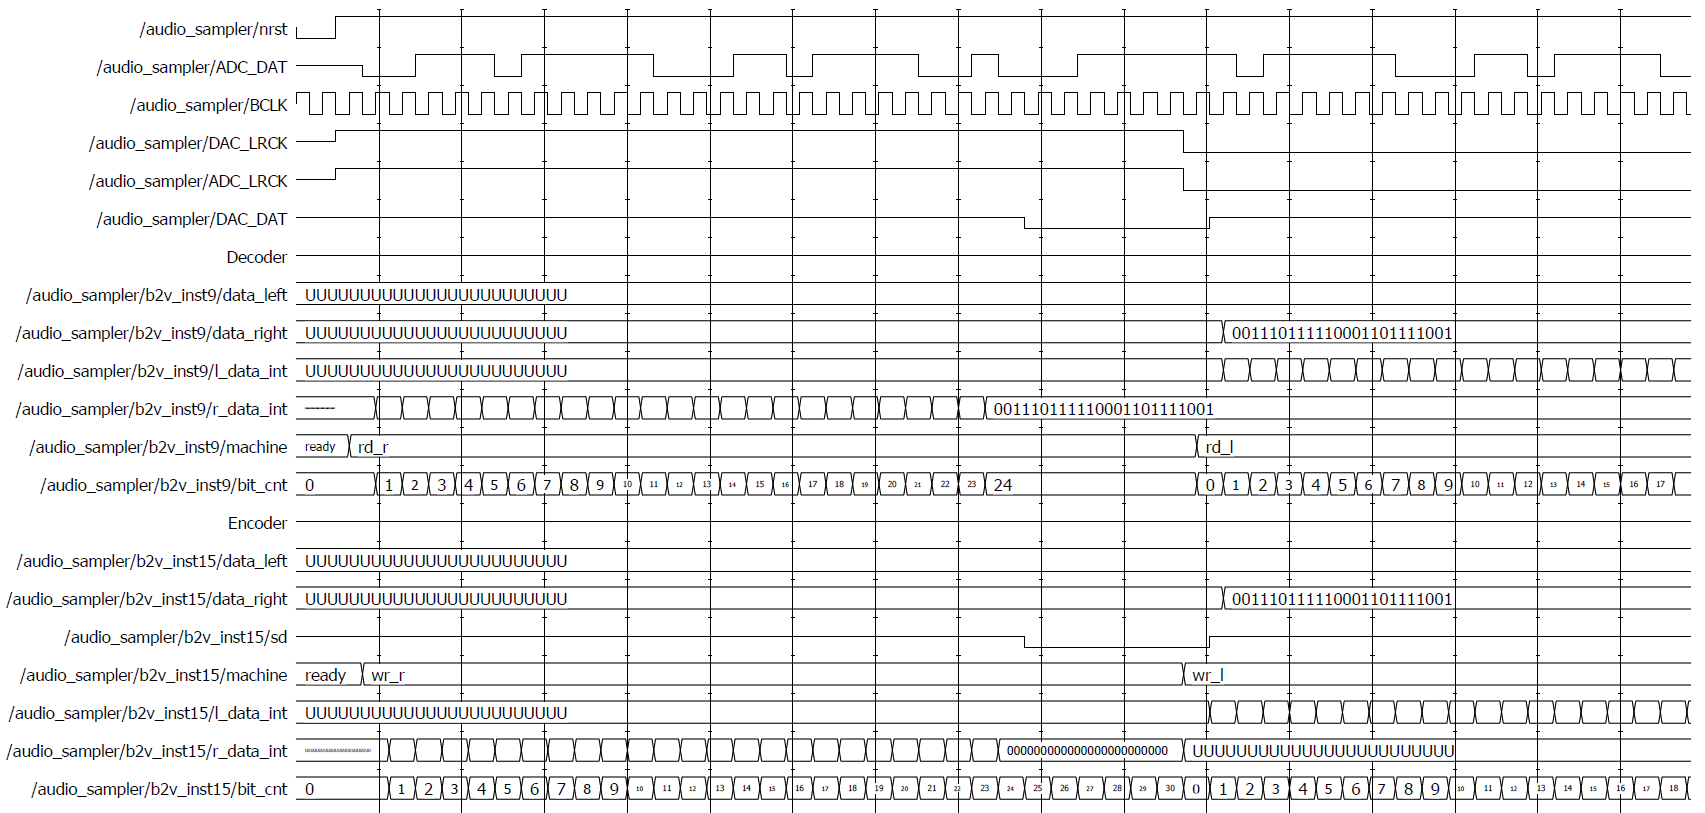
\includegraphics[width=\linewidth, keepaspectratio]{Audio_sampler_result.png}
    \caption{Simulation result of I2S decoder and encoder}
    \label{fig:i2s-dec-enc}
\end{figure}

\subsubsection{I2C master}
The results can be seen in figure \ref{fig:i2c-master}. In this result it can be seen that the I2C master works as expected according to the protocol standards.

\begin{figure}[!ht]
    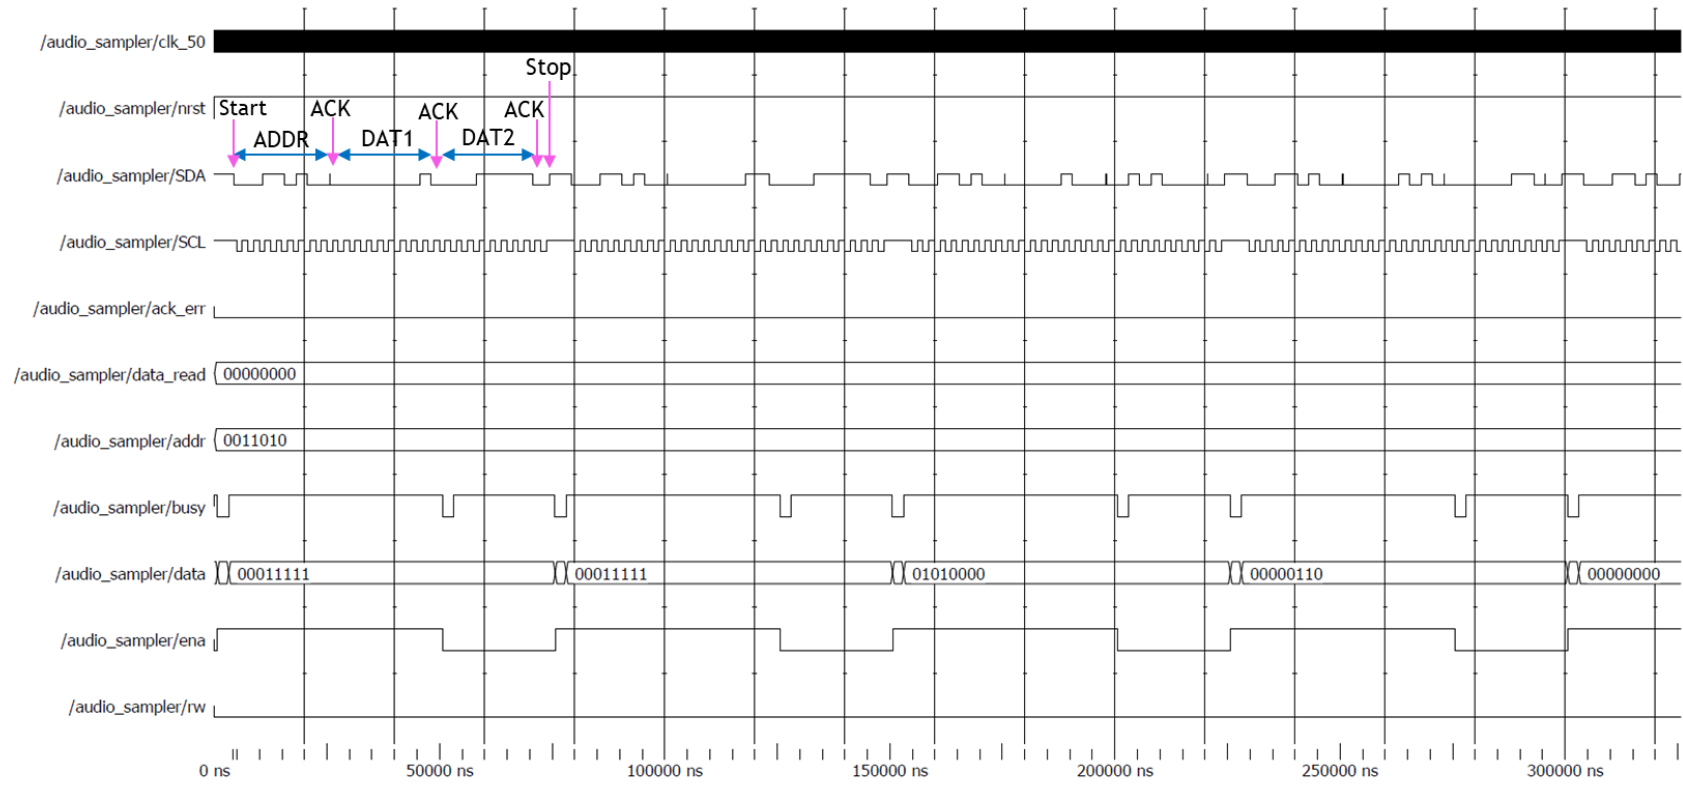
\includegraphics[width=\linewidth, keepaspectratio]{I2C_master_result.png}
    \caption{Simulation result of I2C master}
    \label{fig:i2c-master}
\end{figure}

\subsubsection{State-space BPF}
Due to time constrains the BPF has not yet been tested in Multisim. 

\section{Conclusions}

\subsection{Hardware}

\subsubsection{Buck}
Due to the limited time, this verification has not been done yet.

\subsubsection{SEPIC}
The SEPIC appears to be functioning well after some quick measurements. With an input voltage of +12V, it generates a stable -15V output voltage, and the voltage ripple remains nearly constant regardless of the output current. This aligns with the calculations and simulations. Additionally, the amplitude of the output ripple voltage closely matches the calculated and simulated values.

\subsubsection{Linear voltage regulator}
Due to the limited time, this verification has not yet been completed.

\subsubsection{Main board}
Due to the limited time, this verification has not been done yet.

\subsection{Firmware}
The I2S decoder, I2S encoder and I2C master work as expected. Therefore it is possible to sample audio using the ADC and DAC of the FPGA board. This has been tested and verified that this works. 

Due to time constrains further testing and implementation of the effects has not been conducted. 
